\begin{tikzpicture}[auto,scale = 0.7]
\draw (0,0.5) -- (3,0.5);
\draw (0.5,0.4) -- (0.5,0.6);
\node at (0.5,1) {0};
\node at (2.5,1) {1};
\node at (2.5,0.5) {$\bullet$};
\end{tikzpicture}
\begin{tikzpicture}
\draw[color = white] (0,-1) rectangle (0.7,-2);
\end{tikzpicture}
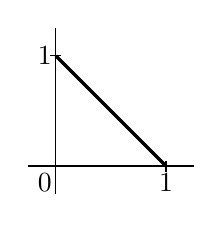
\begin{tikzpicture}[auto,scale = 0.7]
\draw (-0.5,0) -- (2.5,0);
\draw (0,-0.5) -- (0,2.5);
\draw (2,-0.1) -- (2,0.1);
\draw (-0.1,2) -- (0.1,2);
\node at (-0.2,-0.3) {0};
\node at (2,-0.3) {1};
\node at (-0.2,2) {1};
\draw [very thick] (2,0) -- (0,2);
\end{tikzpicture}
\begin{tikzpicture}
\draw[color = white] (0,-1) rectangle (0.7,-2);
\end{tikzpicture}
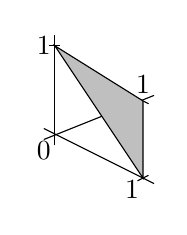
\begin{tikzpicture}[auto,scale = 0.7]
\draw (0,0) -- (0,2);
\draw (-0.2,0.1) -- (1.8,0.9);
\draw (-0.2,0.3) -- (1.8,-0.7);
\node at (-0.2,-0.1) {0};
\draw (-0.1,1.8) -- (0.1,1.8);
\node at (-0.2,1.8) {1};
\draw (1.5,-0.65) -- (1.7,-0.55);
\node at (1.4,-0.80) {1};
\draw (1.5,0.85) -- (1.7,0.75);
\node at (1.6,1.1) {1};
\draw[fill = gray!50] (0,1.8) -- (1.6,-0.6) -- (1.6,0.8) -- cycle;
\end{tikzpicture}
\begin{tikzpicture}
\draw[color = white] (0,-1) rectangle (0.7,-2);
\end{tikzpicture}
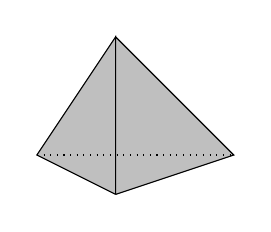
\begin{tikzpicture}[auto,scale = 1]
\node (0) at (0,0) {};
\node (1) at (-1,0.5) {};
\node (2) at (1.5,0.5) {};
\node (3) at (0,2) {};
\draw[fill = gray!50] (0,0) -- (-1,0.5) -- (0,2) -- (0,0);
\draw[fill = gray!50] (0,0) -- (1.5,0.5) -- (0,2) -- (0,0);
\draw[dotted] (-1,0.5) -- (1.5,0.5);
\end{tikzpicture}